\section{Theory of Operations}

\subsection{Introduction}
The \textbf{DynamicFifo} is a highly parameterized FIFO and FIFO controller. It
is configurable as a full self-contained FIFO with internal memory being
constructed from flip-flops, or a FIFO controller that uses an external SRAM
for memory.

\begin{figure}[h]
  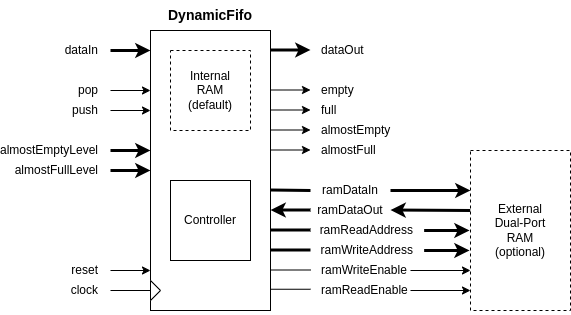
\includegraphics[width=0.80\textwidth]{images/block-diagram.png}
  \caption{Block Diagram}\label{fig:block-diagram}
\end{figure}

It features the following status flags which are described in
Table~\ref{table:ports}.

\begin{itemize}[noitemsep]
  \item{empty}
  \item{full}
  \item{almostEmpty}
  \item{almostFull}
\end{itemize}

When \textit{push} is asserted, the data on the \textit{dataIn} port is enqued
on the next rising edge of \textit{clock}. When \textit{pop} is asserted, the
top of the FIFO is dequed and immediately available on the \textit{dataOut}
port. Pop and Push operations can be simulataneous.

There are two error conditions which produce the following effects:
\begin{itemize}
  \item{When \textit{pop} is asserted and the FIFO is empty (\textit{empty} is
        active), \textit{dataOut} will contain the last valid data held in
        the FIFO.}
  \item{When \textit{push} is asserted and the FIFO is full (\textit{full} is
        active), \textit{dataIn} will be ignored and not enqued.}
\end{itemize}

The \textit{almostEmpty} and \textit{almostFull} flags allow for additional
feedback to the system that is useful for optimizing data flow control. The
levels of these flags can be programmed dynamically through the
\textit{almostEmptyLevel} and \textit{almostFullLevel} ports.

\newpage
\subsection{Interface Timing}

GPIO has a synchronous APB3 interface, and a GPIO interface. The timing diagram shown below
in Figure~\ref{fig:timing} represents an instantiation with the following
parameters.

\begin{lstlisting}[language=Scala]
val myGPIO = new GPIO(
  dataWidth = 16, 
  addrWidth = 16 ) 
\end{lstlisting}

\begin{figure}[h]
  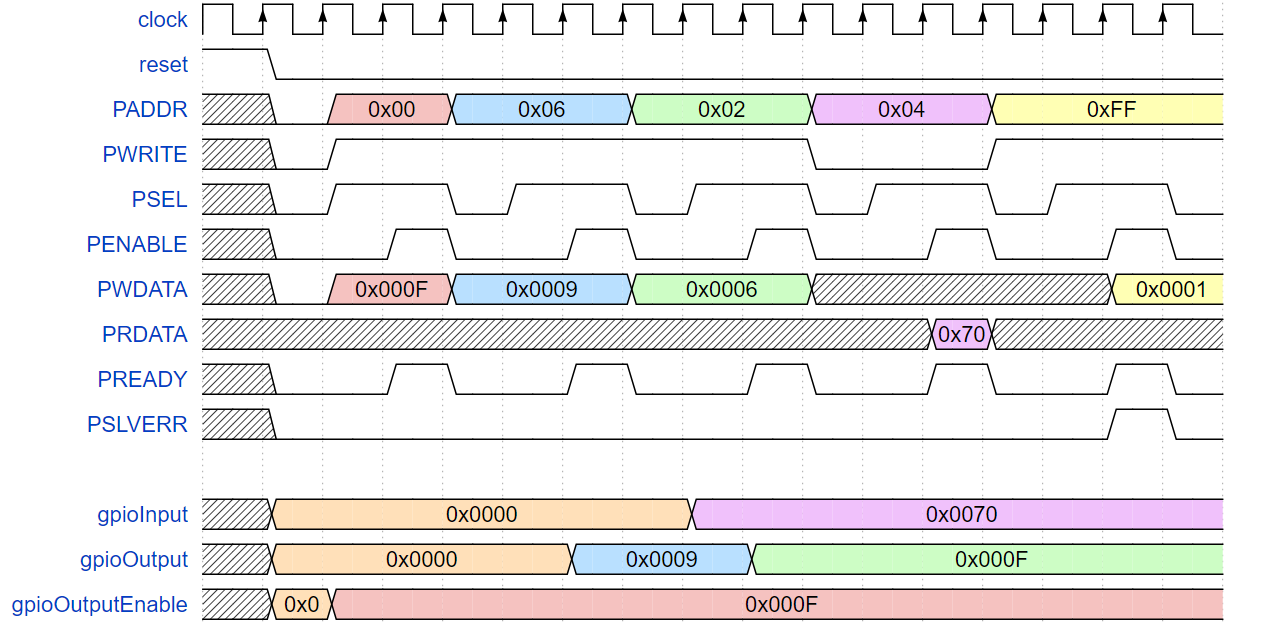
\includegraphics[width=\textwidth]{images/GPIO-timing.png}
  \caption{Timing Diagram}\label{fig:timing}
\end{figure}

This shows the operation of the basic read/write register operations following the APB protocol. Registers DIRECTION, MODE, and OUTPUT are
written to, while register INPUT is read from.

The \textit{gpioOutputEnable} port is driven to a value of 0x000F after 0x000F is written to the DIRECTION register 
at address 0x00. Next, the MODE register at address 0x06 is written a value of 0x0009. The \textit{gpioOutput} port 
then has a value of 0x0009 because of the open-drain mode operation. 

The OUTPUT register is then written a value of 0x0006 at address 0x02. \textit{gpioOutput} takes on a value of 0x000F
since the MSB and LSB are operating on open-drain mode, and the middle two bits are operating on push-pull mode. 

The INPUT register is read from at address 0x04, which has a value of 0x0070 since \textit{gpioInput} has a value fo 0x0070.
On the final transaction, PSLVERR goes high because an invalid address is written to.